\section{Model methodologie}\label{Sect_Methodologie}
\subsection{Incurred but not reported}
	The task of the actuarial model is to predict the IBNR, the incurred but not reported claims. The IBNR can be divided into 3 distinct elements, which we defined as pure IBNR, IBNER and IBNR on reopen. Pure IBNR are claims which are not reported at the observation date, meaning the insurer has no information on them. The insurer only knows that a claim happened when it is reported. IBNER, incurred but not enough reported, are claims which have been reported and the insurer has information on the claims in their database. IBNR on reopen consist of closed claims which might reopen at any given time. This mean that a claim which closed in 2017 might reopen in 2018 or 2019. IBNR on reopen is a small proportion of the total IBNR, but still should be considered in the model. Figure \ref{Fig_IBNER_timeline} gives a visual representation of these categories. 
	\begin{figure}[H]
		\begin{center}
			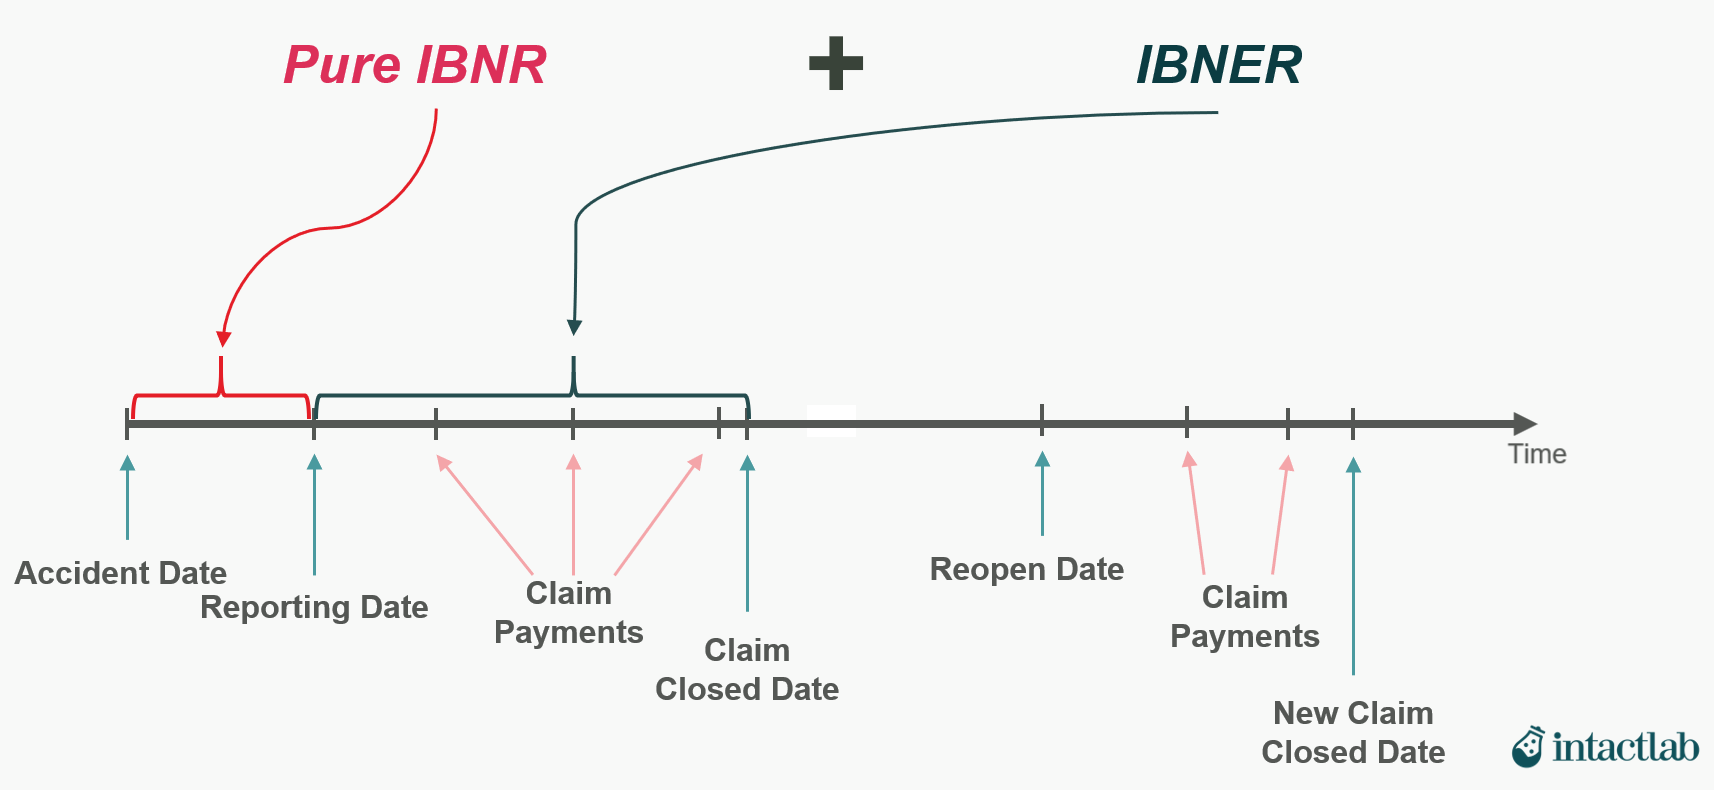
\includegraphics[scale=0.2]{Graphiques/IBNER_timeline} 
			\renewcommand{\figurename}{Figure}
			\caption{Timeline of a claim}\label{Fig_IBNER_timeline}
		\end{center}
	\end{figure}

\subsection{Hierarchical approach}
	The actuarial department uses a modified chain-ladder method for their model. This model uses a more hierarchical approach, where the data is clustered into more homogeneous groups. First, we develop a model for each of the three IBNR types. The claims team focuses on the IBNER part, while the pure and IBNR on reopen models are still chain-ladder based and were developed by the actuarial department. For the IBNER model, we grouped the data according to the following claims characteristics, called \texttt{leaf}:  total loss (\texttt{43}), total loss without replacement cost endorsement (\texttt{n43}), luxury repairable vehicles (\texttt{rep\_lux}), non-luxury non-rental repairable vehicles (\texttt{rep\_nlux\_nrent}) and non-luxury rental repairable vehicles (\texttt{rep\_nlux\_rent}). We suppose that the frequency and severity distributions are very similar within these groups. Figure \ref{Fig_hier_model} gives an overview of the hierarchical approach, including small statistics.
	\begin{figure}[H]
		\begin{center}
			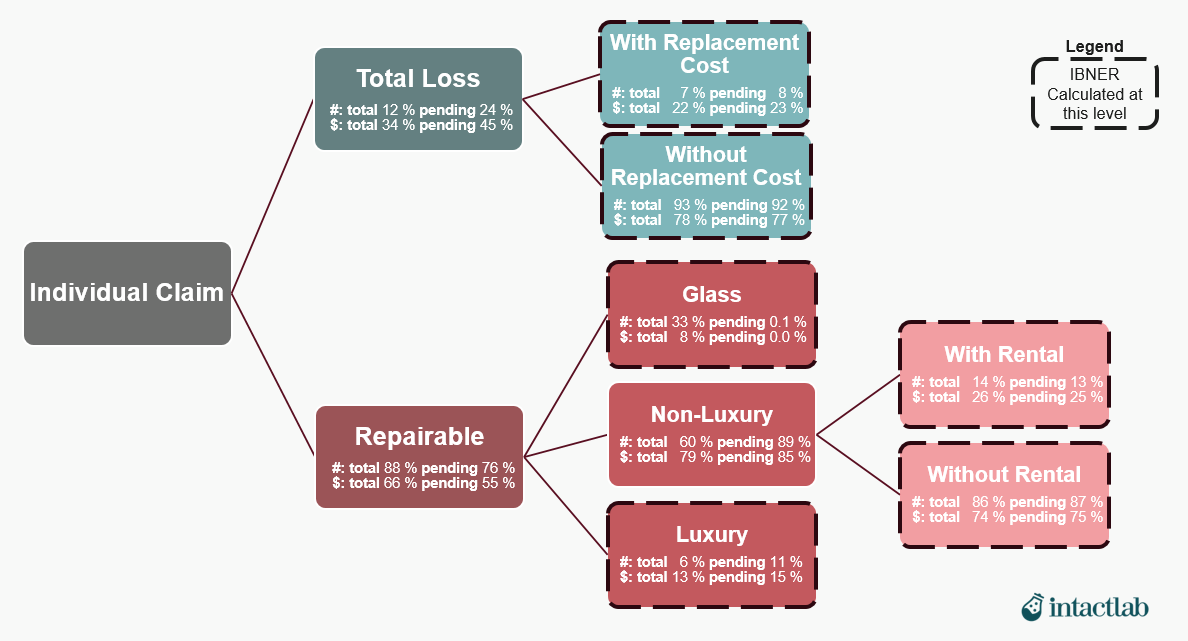
\includegraphics[scale=0.4]{Graphiques/Hier_model} 
			\renewcommand{\figurename}{Figure}
			\caption[Hierarchical model structure]{Hierarchical model structure. The statistics give the percentage proportion of claims in number of claims (\#) and in dollars amount (\$). The total percentage is based on the previous subgroup total. The pending percentage is based on the pending of the previous subgroup.}\label{Fig_hier_model}
		\end{center}
	\end{figure}
 
\subsection{Key formulas}
	As mentioned in section \ref{Section_dataAnalysis}, the \texttt{ACV} and \texttt{GAV} have strong predictive strength. We use a basic formula to link the \texttt{GAV}/\texttt{ACV} with the ultimate and use historical information of claims.

	 
	\begin{Definition}
		We define $\hat{L}_i$ as ultimate loss prediction for claims pending/open in period $i$ and $X_i$ as the predictor, in our case \texttt{GAV} or \texttt{ACV} used to predict period $i$. Their relationship is defined as
		$$\hat{L}_i = \hat{\Theta}_i \times X_i,$$
		where $\hat{\Theta}_i$ is the factor for the time period $i$.
	\end{Definition}
	We need to calculate the factor $\hat{\Theta}_i$ with the available historical data. 
	\begin{Definition}
		We define $\widetilde{L}_{j,i}$ as total incurred for claims in the time period $j$ as of $i$. $X_j$ is the predictor in the time period $j$. Thus, the factor is defined as
		$$\hat{\theta}_i = \frac{\widetilde{L}_{j,i}}{X_j}.$$
	\end{Definition}

	Note the difference between $\hat{L}_i$ and $\widetilde{L}_{j,i}$. The former is the ultimate we want to predict, so we do not know its value in observation month $i$. The latter is the total incurred for claims in period $j$ we know as of $i$. For illustration in the sample data of figures \ref{Fig_sample_1} and \ref{Fig_sample_2}, we want to calculate the factor $\hat{\theta}_{201804}$. We suppose we want to use open claim with $ \texttt{CLM\_NBR} = 123456789$ to calculate this factor, then 
	\begin{align*}
	\widetilde{L}_{201711, 201804} &= \texttt{AUTO\_LTD\_NET\_LOSS\_PAID\_AMT} + \texttt{AUTO\_LTD\_ALAE\_INCURRED\_AMT} \\
									& \ \ \	+ \texttt{AUTO\_LTD\_LOSS\_RES\_CHG\_AMT} \\
									&= 11213.87
	\end{align*}
	 as of $201804$ ($\texttt{obs\_month} = 201804$) and $X_j = \texttt{AvgTypicalCarValue} = 8007 $.
	As the example illustrated, the ultimate and the predictor are historical values which should be fully developed. It is necessary to have a least 5 to 12 months of development, so that the factors are stable enough. The difference in time between the moment we want to predict the pending and the historical data, $i - j$ is defined as the lag. How many historical observation month $j$ we use for the calculation is defined as period length. Figure \ref{Fig_lag_pl} shows a 5-month lag and 3-month period length. We want to predict the ultimate of the December 2018, $i = 201812$ pending (open) claims. We go back 5 months and use the historical claim data from open claims in May, June and July 2018, $j=201805, 201806, 201807$. This means that their \texttt{sf\_status} needs to be either "OP" for open or "RO" for reopen in the observation month $j=201805, 201806, 201807$.
	\begin{figure}[H]
		\begin{center}
			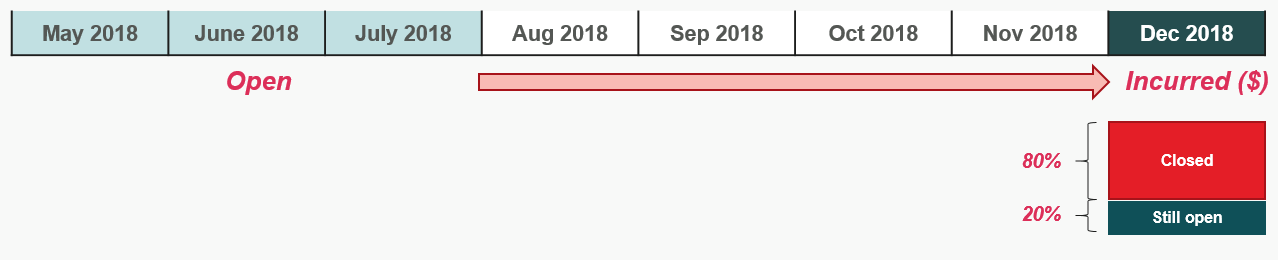
\includegraphics[scale=0.4]{Graphiques/lag_pl} 
			\renewcommand{\figurename}{Figure}
			\caption{Lag and period length visualization}\label{Fig_lag_pl}
		\end{center}
	\end{figure}
	This approach is similar to a lagged moving average model. We use the incurred as of December 2018 of claims that are open at least once in May, June and July. Thus, the incurred had a minimum of 5 months to develop. Then, we divide this incurred by the aggregated \texttt{GAV} or \texttt{ACV} in May, June and July. We only keep the most recent data line for each claim, in other words, we don’t have any duplicates per claim number. Figure \ref{Fig_factor_example} gives a numerical example. 
	\begin{figure}[H]
		\begin{center}
			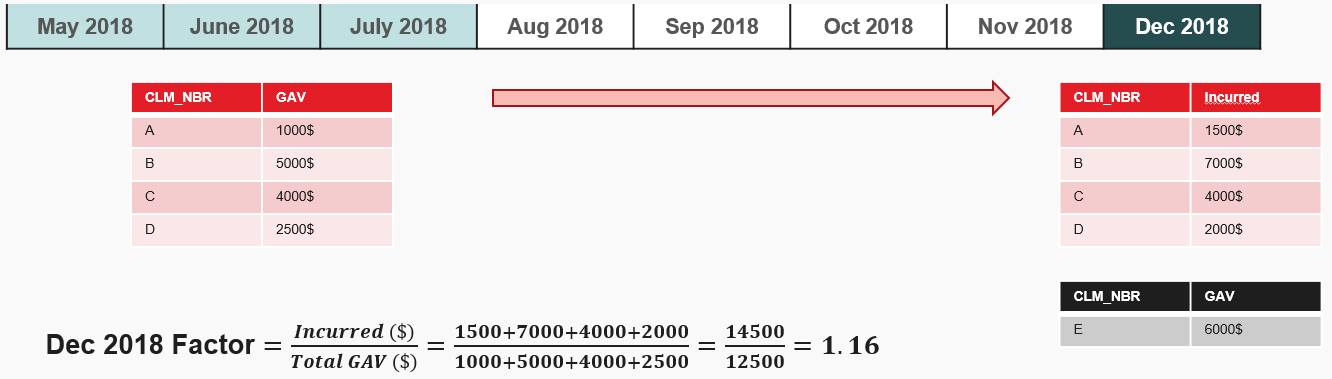
\includegraphics[scale=0.4]{Graphiques/factor_example} 
			\renewcommand{\figurename}{Figure}
			\caption{Factor calculation example}\label{Fig_factor_example}
		\end{center}
	\end{figure}
	Note that in figure \ref{Fig_lag_pl} the incurred is subdivided into open and closed claims, since it is possible that claims remain open even after 5 months. Therefore, we calculate a claim number weighted average of closed and open factors. As final factor we get definition \ref{Def_final_factor}.
	\begin{Definition}\label{Def_final_factor}
		$\hat{\Theta}_i$ is the final factor used for the prediction. $\hat{\theta}_{i,open}$ is the factor for claims that are still open during $i$ and  $\hat{\theta}_{i,closed}$ is the factor for claims that are closed during $i$. Furthermore, $n_{open}$ is the number of open claims in period $i$ and $n_{closed}$ is the number of closed claims in period $i$. Thus, we have
		$$\hat{\Theta}_i = \frac{n_{open}}{n_{open} + n_{closed}} \hat{\theta}_{i,open} + \frac{n_{closed}}{n_{open} + n_{closed}}  \hat{\theta}_{i,closed}.$$ 
	\end{Definition}
	
	We multiply this factor by the aggregated \texttt{GAV} or \texttt{ACV} of pending claims (December 2018 in the previous example) to get the ultimate amount.
	
	\begin{Definition}\label{Def_IBNER}
		We define the $IBNER$ in period $i$ as
		$$IBNER_i = \hat{L}_i - I_i,$$
		where $I_i$ is the incurred payments and reserve for claims pending in period $i$.
	\end{Definition}
	Note that once claims are fully developed $L_i = I_i$, where $L_i$ is the real observed ultimate loss for claims open in period $i$. 
	The prediction results for the model are discussed in section \ref{Sect_Results}.
	
\subsection{Imputation methodology}
	It is important to note that no data is perfect. The dataset contains a non-negligible amount of missing \texttt{GAV} and \texttt{ACV} values. About 17\% of the claims have missing \texttt{GAV} or \texttt{ACV}, some regions and line of business are worse than others. Figure \ref{Fig_imputation_example} demonstrates how missing values are imputed. If we have missing values, we calculate the median of the existing values in the time window. We replace the missing values by the median and execute the factor calculations without any further readjustment. This method is not perfect and should be revised. For instance, in the previous example, we would overestimate the factor since we impute with a lower value.  
	\begin{figure}[H]
		\begin{center}
			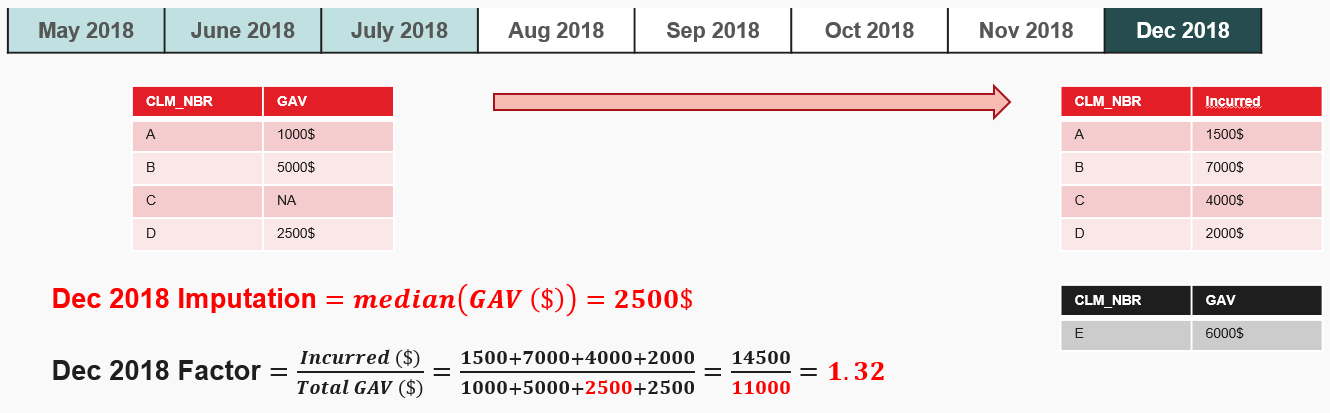
\includegraphics[scale=0.4]{Graphiques/imputation_example} 
			\renewcommand{\figurename}{Figure}
			\caption{Factor calculation example with missing values}\label{Fig_imputation_example}
		\end{center}
	\end{figure}

\subsection{Adjusting the lag and period length}\label{Sect_dec_march}
As we have noticed in the analysis of the data, Alberta clearly has different patterns than the other regions. Claims in Quebec and Ontario settle considerably faster (after 4-5 months) and recovery is less impactful. Note that in section \ref{Sect_Results}, figure \ref{Fig_IBNER_preds}, we have an December 2019 and an March 2020 model. The main different between the two are the Alberta hyper-parameters. In December 2019, all regions had the same lag of 5 months. A more detailed analysis shows an advantage to increase the lag for Alberta to 10 months.  In Alberta having a lag of 5 is clearly insufficient, thus using a lag of 10 is necessary. This gives the claims at least 10 months to fully develop. In addition, a lag and period length that includes the 12th month, is beneficial if we have seasonal effects.

\subsection{Second model iteration: Historical pending but now closed claims}
After having used the first iteration of the model for December 2020 and March 2020. We noticed systematic error, i.e. constant over- or underestimation. This might be related to the open claims (after the lag) which are used to calculate the factors. Since open claims still have a case reserve, the incurred used for the factor might be inflated, thus explaining overestimation. Indeed, the factor for open claims is always larger than the factor for closed. If we overestimate constantly, we attribute too much weight to still open claims. In the second iteration of the model, we discard the weighted average and we only use the factor of closed claims. In short, based on definition \ref{Def_final_factor}, we have
$$\hat{\Theta}_i = \hat{\theta}_{i,closed}.$$
This also has the benefit that closed claims usually should not develop further and thus have less volatility in the calculation of the factors. The results are discussed in section \ref{Sect_Results}.
\subsection{Third model iteration: Historical closed claims}
The final iteration of the model is based on the idea of the second iteration. The idea is to only use closed claims. However, in the second iteration we use the factor of closed claims of the lagged 3-month period, while in this iteration we want to increase the number of claims used in the calculations and add more recent claims. Consequently, instead of using the pending claims in a historical time window, we calculate factors for all claims that closed in the time window. This simply implies changing the filter on \texttt{sf\_status}. If we have used the previous example, we want to predict the pending claims in December 2018, we use all claims that closed between May and July for the factor calculations. Since the claims are closed, it is unlikely that we have still open claims in December.
